
Every locally semicomplete digraph can be classified into some other groups of digraphs, namely semicomplete digraphs and round decomposable digraphs and the last one which is neither of the two is called evil (a name first introduced in \cite{bangJGT85} and will be defined more precisely towards the end of this section). 
Round-decomposable digraph $D=R[D_1,\dots,D_r]$ is where $R$ is a round digraph of the strong semicomplete digraphs $D_i$ and $|R|=r$.
In \autoref{sec:class} there was a briefly definition of round digraph for a more formal definition we use the definition from \cite{bangJGT77}.
\begin{definition}~\cite{bangJGT77}
    A digraph on $n$ vertices is round if we can label its vertices $v_1,\dots ,v_n$ so that for each $i$, we have $N^+(v_i)=\lbrace v_{i+1},\dots ,v_{i+d^+(i)}\rbrace$ and $N^-(v_i)=\lbrace v_{i-d^-(i)},\dots ,v_{i-1)}\rbrace$. We call the labeling $v_1,\dots ,v_n$ a round ordering. 
\end{definition}
It turns out the class of locally semicomplete digraph is split up in these 3 subclasses and these subclasses are going to be important for proving a lot of the problems we are going to cover in this thesis.
\begin{thm}~\cite{bangDM167,bangJGT85}
    Let $D$ be a locally semicomplete digraph. 
    Then exactly one of the following possibilities holds.
    \begin{itemize}
        \item[(a)] $D$ is round decomposable with a unique round decomposition $R[D_1,\dots ,D_r]$, where $R$ is a round local tournament on $r\geq 2$ vertices and $D_i$ is strong semicomplete digraph for $i=1,2,\dots,r$.
        \item[(b)] $D$ is evil.
        \item[(c)] $D$ is a semicomplete digraph that is not round decomposable. 
    \end{itemize}
    Furthermore, there is a polynomial algorithm that decides which of the properties holds and gives a certificate for this.
    \label{thm:treesubclasses}
\end{thm}
If the locally semicomplete digraph is nonstrong, it turns out that it is decomposable. 
This is called a semicomplete decomposition. 
\begin{thm}~\cite{bangJGT85,banggutin,bangJCT102}
    Let $D$ be a nonstrong locally semicomplete digraph and let $D_1,D_2,\dots,D_p$ be the acyclic order of the strong components of $D$. Then $D$ can be decomposed into $r\geq 2$ disjoint subdigraphs $D_1',D_2',\dots, D_r'$ as follows:
    \begin{align*}
        D_1'=D_p, \qquad \lambda_1=p,\\
        \lambda_{i+1}=min\lbrace j|N^+(D_j)\cap V(D'_i)\neq \emptyset\rbrace,
    \end{align*}
    and
    \begin{equation*}
        D'_{i+1}=D\left< V(D_{\lambda_{i+1}})\cup V(D_{\lambda_{i+1}+1})\cup \cdots \cup V(D_{\lambda_{i}-1})\right> .
    \end{equation*}
    The subdigraphs $D'_1,D'_2,\dots,D'_r$ satisfy the properties below:
    \begin{itemize}
        \item[(a)] $D'_i$ consists of some strong components that are consecutive in the acyclic ordering of the strong components of $D$ and is semicomplete for $i=1,2,\dots ,r$;
        \item[(b)] $D'_{i+1}$ dominates the initial component of $D'_i$ and there exists no arc from $D'_i$ to $D'_{i+1}$ for $i=1,2,\dots ,r-1$;
        \item[(c)] if $r\geq 3$ then there exists no arc between $D'_i$ and $D'_j$ for $i,j$ satisfying $|j-i|\geq 2$  
    \end{itemize}
    \label{thm:semicompletedecom}
\end{thm}
For simplification of \autoref{thm:semicompletedecom} the properties are drawn out in \autoref{fig:properties}
\begin{figure}
    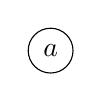
\begin{tikzpicture}[main/.style ={draw,circle}]
        \node[main](a){$a$};
    \end{tikzpicture}
    \caption{(a),(b) and (c)}
    \label{fig:properties}
\end{figure}
If $D$ is a locally semicomplete digraph that is not semicomplete, it can still be strong and if this is the case, we can find a minimum seperator $S$. Since a seperator $S$ make $D-S$ a non-strong digraph, we can make a semicomplete decomposition out of $D-S$.
\begin{thm}~\cite{banggutin}
    If a strong locally semicomplete digraph $D$ is not semicomplete, then there exists a minimal seperating set $S\subseteq V$ such that $D-S$ is not semicomplete. 
    Furthermore, if $D_1,D_2,\dots , D_p$ is the acyclic ordering of the strong components of $D-S$ and $D'_1,D'_2,\dots ,D'_r$ is the semicomplete decomposition of $D-S$, then $r\geq 3$, $D\left<S\right>$ is semicomplete and we have $D_p\mapsto S\mapsto D_1$.  
\end{thm}
Some of them are round-decomposable and we will later see that it is the when $r>3$ in the semicomplete decomposition. 
It also turns out that this round-decomposistion is unique.
\begin{cor}~\cite{bangDM167}
    If a locally semicomplete digraph $D$ is round decomposable, then it has a unique round decomposition $D=R[D_1,D_2,\dots ,D_{\alpha}]$.
\end{cor}
From \autoref{thm:treesubclasses} we know that for a round-decomposable digraph the quotient graph is round and the houses are semicomplete making them totally $\phi_2$-decomposable then by \autoref{thm:phipoly} we know that we can find the decomposition in polynomial time.
\begin{prop}~\cite{bangDM167}
    There exists a polynomial algorithm to decide whether a given locally semicomplete digraph $D$ has a round decomposition and to find this decomposition if it exists.
\end{prop}
Like we briefly meantioned above the locally semicomplete digraph that are not semicomplete and not round have a semicomplete decomposistions on where $r=3$ also those we call evil.
The evil locally semicomplete digraphs are the ones we are focusing on for the rest of this section.
\begin{lemma}~\cite{bangDM167}
    Let $D$ be a strong locally semicomplete digraph which is not semicomplete. 
    Either $D$ is round decomposable, or $D$ has a minimal seperating set $S$ such that the semicomplete decomposition of $D-S$ has exactly three components $D'_1,D_2',D_3'$.
\end{lemma}
There is a good understanding of the structure of round-decomposable and the semicomplete digraphs, even the semicomplete decomposition which is a part of the evil structure too.
We are now going to construct then use this to construct what we call a \textbf{good} seperator.
\begin{lemma}~\cite{bangJGT85}
    Let $S$ be a minimal seperator of the locally semicomplete digraph $D$. 
    Then either $D\left< S\right>$ is semicomplete or $D\left< V-S\right>$ is semicomplete.
    \label{lem:whichsemicomplete}
\end{lemma}
Then a \textbf{good} seperator of a locally semicomplete digraph is minimal and $D\left<S\right>$ is semicomplete.
When finding a good seperator in an evil locally semicomplete digraph, then the part that is left $D-S$ is a non-strong locally semicomplete digraph and we can therefore use \autoref{thm:semicompletedecom} to find the semicomplete decomposition of $D\left<V-S\right>$, it turns out that there is a lot to say about this decomposition. 
With this decomposistion, we can classify the quotient graph but we can try to describe more deeply how it looks.
\begin{thm}~\cite{bangJGT85,bangJCT102}
    Let $D$ be an evil locally semicomplete digraph then $D$ is strong and satisfies the following properties.
    \begin{itemize}
        \item[(a)]There is a good seperator S such that the semicomplete decomposition of $D-S$ has exactly three components $D'_1,D'_2,D'_3$ (and $D\left<S\right>$ is semicomplete by \autoref{lem:whichsemicomplete});
        \item[(b)] Furthermore, for each such $S$, there are integers $\alpha, \beta,\mu,\nu$ with $\lambda_2\leq \alpha \leq \beta \leq p-1$ and $p+1\leq \mu \leq \nu \leq p+q$ such that 
        \begin{align}
            &N^-(D_\alpha)\cap V(D_\mu)\neq \emptyset \text{ and } N^+(D_\alpha)\cap V(D_\nu)\neq \emptyset,\\
            \text{or } &N^-(D_\mu)\cap V(D_\alpha)\neq \emptyset \text{ and } N^+(D_\mu)\cap V(D_\beta)\neq \emptyset,
        \end{align} 
        where $D_1,D_2,\dots, D_p$ and $D_{p+1},\dots,D_{p+q}$ are the strong decomposition of $D-S$ and $D\left< S\right>$, respectively, and $D_{\lambda_2}$is the initial component of $D'_2$. 
    \end{itemize}
    \label{thm:evildecom}
\end{thm}
Even though this is a structure we can work with, we can actually go deeper into the structure of this evil locally semicomplete digraph. 
Namely trying to group the components inside the semicomplete decomposition $D'_1,D'_2,D'_3$ and the good seperator $S$. 
This structure is mentioned in \cite{bangJGT85} but also in \cite{tildeDMCS}. 
First we can establish lemma, which is a big part of the structure of evil locally semicomplete digraphs.
\begin{lemma}~\cite{tildeDMCS}
    Let $D$ be an evil locally semicomplete digraph and let $S$ be a good seperator of $D$. 
    Then the following holds:
    \begin{itemize}
        \item[(i)] $D_p\Rightarrow S\Rightarrow D_1$.
        \item[(ii)] If $sv$ is an arc from $S$ to $D'_2$ with $s\in V(D_i)$ and $v\in V(D_j)$, then 
        \begin{equation*}
            D_i\cup D_{i+1}\cup \dots D_{p+q}\Rightarrow D_1\cup\dots \cup D_{\lambda_2-1}\Rightarrow D_{\lambda_2}\cup \dots \cup D_j.
        \end{equation*}
        \item[(iii)] $D_{p+q}\Rightarrow D'_3$ and $D_f\Rightarrow D_{f+1}$ for $f\in [p+q]$, where $p+q+1=1$.
        \item[(iv)] If there is any arc from $D_i$ to $D_j$ with $i\in [\lambda_2-1]$ and $j\in [\lambda_2,p-1]$, then $D_a\Rightarrow D_b$ for all $a\in [i,\lambda_2-1]$ and $b\in[\lambda_2,j]$.
        \item[(v)] If there is any arc from $D_k to D_l$ with $k\in [p+1,p+q]$ and $l\in [\lambda_2-1]$, then $D_a\Rightarrow D_b$ for all $a\in [k,p+q]$ and $b\in [l]$.   
    \end{itemize}
\end{lemma}
